\chapter{Procesamiento de imágenes}\label{procesamiento-de-imagenes}

El procesamiento digital de imágenes (PDI o DIP por sus siglas en
inglés) es un campo de investigación científica muy interesante y cuyas
aplicaciones son tan diversas, tales como la medicina, el control de
calidad en la industria, astronomía, visión artificial, etc. Lo anterior
nos hace deducir que para abarcar ``decentemente'' la mayoría de los
tópicos comunes del PDI se necesitaría más de un libro completo, por lo
cual se pretende aclarar que en este capítulo se tratarán solamente
algunos temas con un nivel de detalle elemental, con la esperanza de que
sirva al amable lector como una breve introducción y sobre todo, en
medida de lo posible, motivarle para adentrarse en tan maravilloso mundo.

\section{Conceptos iniciales del procesamiento de imágenes}

\subsection{¿Qué es el procesamiento de imágenes?}

El procesamiento digital de imágenes es el conjunto de técnicas
aplicadas a imágenes digitales con un cierto objetivo, los cuales pueden
ser: mejorar la calidad de la imagen, detección/reconocimiento de formas
o colores, realce de ciertas regiones de la imagen, etc.

\subsection{Aplicaciones del procesamiento de imágenes}

\section{Importar y mostrar imágenes}

En MATLAB, como en cualquier otro software de procesamiento, las
imágenes son tratadas como matrices, cuyos elementos corresponden a un
valor especifico de cada píxel que la compone. La función
\texttt{imread} permite leer/importar imágenes en casi cualquier formato
conocido (\emph{.bmp, }.png, \emph{.tiff, }.jpg, etc). La sintaxis de
\texttt{imread} es muy simple, basta con pasar como argumento la
dirección absoluta o relativa del archivo correspondiente a la imagen de
interés, por ejemplo la siguiente instrucción lee la imagen ``img.jpg''
ubicada en la carpeta de trabajo (Current Folder).

\begin{matlab}
>> A=imread('img.png');
\end{matlab}

Con el comando \texttt{whos} podemos verificar el tipo de dato con el
cual MATLAB guarda la imagen importada:

\begin{matlab}
>> whos
  Name        Size                Bytes  Class    Attributes
  A         300x400x3            360000  uint8    
\end{matlab}

MATLAB guarda la información del color de cada píxel que compone la
imagen utilizando una matriz de tres dimensiones; las dos primeras
determinan el tamaño de la imagen y la tercera corresponde a cada una de
las capas RGB, es decir, en una matriz de mxn elementos se guarda la
información correspondiente al color rojo, en otras similares las de
color verde y azul. Por defecto el tipo de dato utilizado para la
manipulación de imágenes es el uint8 (sin signo de 8 bits). \\

Para mostrar una imagen que ha sido previamente leída con \texttt{imread} se
puede utilizar la función \texttt{imshow}. Véase el siguiente ejemplo:

\begin{matlab}
>> A=imread('imag.jpg');
>> imshow(A);
\end{matlab}

\begin{figure}[htbp]
    \centering
    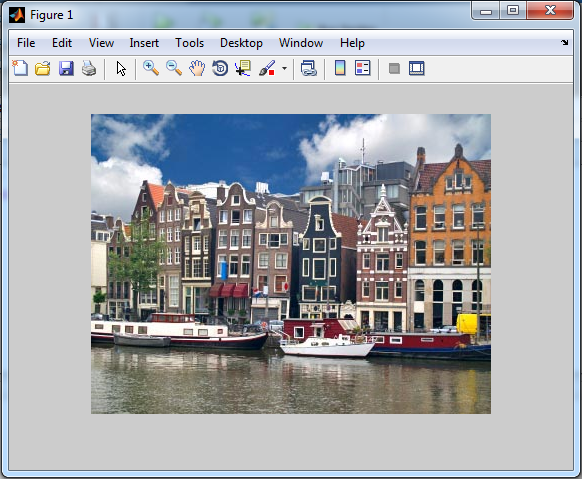
\includegraphics[width=0.75\textwidth]{images/ch7/holland_imshow.png}
    \caption{Utilizando \texttt{imread} e \texttt{imshow}}
    \label{fig:holland_imshow}
\end{figure}


La función \texttt{imshow} abre una nueva ventana (figure) y muestra la
imagen que ha sido guardada con anterioridad (ver figura \ref{fig:holland_imshow}). 
MATLAB dispone de otras funciones como \texttt{image} e \texttt{imagesc} que también muestran en pantalla las
imágenes, pero que suelen utilizarse más para la visualización en
análisis de datos.

\section{Operaciones básicas con imágenes}

\subsection{Operaciones aritméticas}

Recuerde que una imagen en MATLAB se almacena como una matriz de mxnxp
dimensiones, luego, es posible realizar operaciones aritméticas de suma,
resta y multiplicación sobre ella como una matriz común, tal como se ha
visto en Capítulo 2.

\subsubsection{Suma de un escalar}

Si sumamos una constante k a una matriz \textbf{A}, entonces cada
elemento de \textbf{A} se incrementa en k unidades, lo cual se
traduciría en un aumento del brillo en la imagen. Véase el ejemplo
siguiente:

\begin{matlab}
A=imread('imag.jpg');
k=50;
A=A+k;
imshow(A);
\end{matlab}

\begin{figure}[htbp]
    \centering
    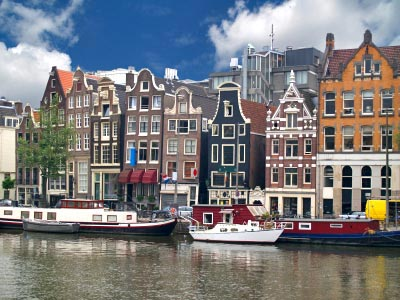
\includegraphics[width=0.75\textwidth]{images/ch7/holland_original.png}
    \caption{Imagen original}
    \label{fig:holland_original}
\end{figure}

\begin{figure}[htbp]
    \centering
    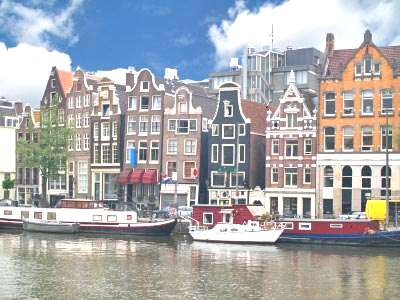
\includegraphics[width=0.75\textwidth]{images/ch7/holland_mas50.png}
    \caption{Imagen aumentada en 50 unidades}
    \label{fig:holland_mas50}
\end{figure}

La imagen \ref{fig:holland_original} corresponde a la original y en
la \ref{fig:holland_mas50} se muestra lo que resulta de aumentar
en 50 unidades cada uno de los pixeles que componen la imagen.

\subsubsection{Resta de un escalar}

Es evidente que la resta de un escalar es muy similar en interpretación
a la suma vista anteriormente, solo que en este caso cada elemento de la
matriz disminuye en un valor constante. Véase el ejemplo:

\begin{matlab}
A=imread('img.jpg');
k=80;
A=A-k;
imshow(A);
\end{matlab}

\begin{figure}[htbp]
    \centering
    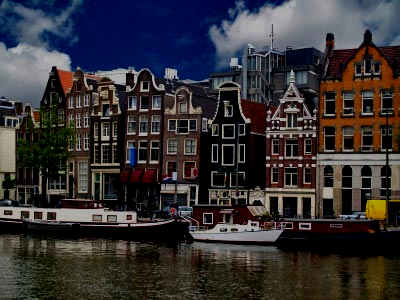
\includegraphics[width=0.75\textwidth]{images/ch7/holland_menos50.png}
    \caption{Imagen disminuida en 50 unidades}
    \label{fig:holland_menos50}
\end{figure}

\subsection{Conversión a escala de grises}

La escala de grises es una forma de representar imágenes digitales
utilizando solamente variaciones de grises, desde negro a blanco. \\

En MATLAB se dispone de la función \texttt{rgb2gray} para convertir una
imagen dada en el modelo de color RGB a una imagen en escala de grises.

\begin{matlab}
X=imread('img.png');
XG=rgb2gray(X);
imshow(XG);
\end{matlab}


\begin{figure}[htbp]
    \centering
    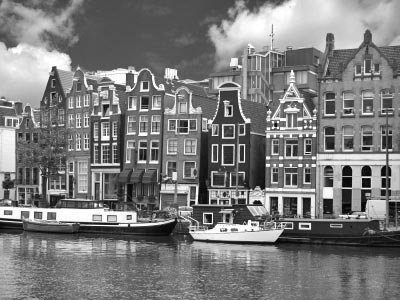
\includegraphics[width=0.75\textwidth]{images/ch7/holland_gris.png}
    \caption{Imagen en escala de grises}
    \label{fig:holland_gris}
\end{figure}

\subsection{Binarización de una imagen}

\subsection{Umbralización}\label{umbralizaciuxf3n}

\subsection{Detección de bordes}\label{detecciuxf3n-de-bordes}

\subsection{Removiendo ruido}\label{removiendo-ruido}